\chapter{Experiments and Results}
\label{chapter6}

In this section, we will describe how we do the experience and the final result of our GEC system. In the experiment part, we mainly train the seq2seq model, do test by applying sample sentence and analysis the model structure and performance.

\section{Experiment Environment}
The software and hardware environments are shown in the following table:
\begin{table}[ht]
\centering
\begin{tabular}{|c | c |} 
    \hline
    GPU & NVIDIA TITAN V $\times2$ \\  
    \hline
    Operating System & Ubuntu 16.04.6 LTS \\ 
    \hline
    Python Version & 3.5.2 (must be this version) \\
    \hline
    Libraries & tensorflow 0.12.0, nltk, pandas, scikit-learn, collections \\ 
    \hline
\end{tabular}
\caption{Environment}
\label{table:1}
\end{table}

\section{Parameters}
The dataset consists of 304,713 lines from movie scripts, of which 243,768 lines were used to train the model and 30,474 lines each were used for the validation and testing sets. The sets were selected such that no lines from the same movie were present in both the training and testing sets.
The model being evaluated below is a sequence-to-sequence model, with attention, where the encoder and decoder were both 2-layer, 512 hidden unit LSTMs. The model was trained with a vocabulary of the 2k most common words seen in the training set.
\section{Performance evaluation}
In the experiment, we run a base line and our model. Here, the baseline is the identity function, which means that we assume no errors exist in the input. To evaluate the performance of the developed GEC system, we apply BLEU score. BLEU score is an algorithm for evaluating the quality of text which has been machine-translated from one natural language to another. The closer the output sentence is to the correct on, the higher the BLEU score is.

The formulation of BLEU score is defined as below.
\begin{align}
    \text{BLEU}=\min(1, \frac{\text{output length}}{reference length})(\prod_{i=1}^{4}\text{precision}_{i})^{\frac{1}{4}}
\end{align}

We sample the sentence from the testing dataset to check the performance. The result is shown in the following.
\begin{figure}
\centering
\begin{subfigure}{.5\textwidth}
    \centering
    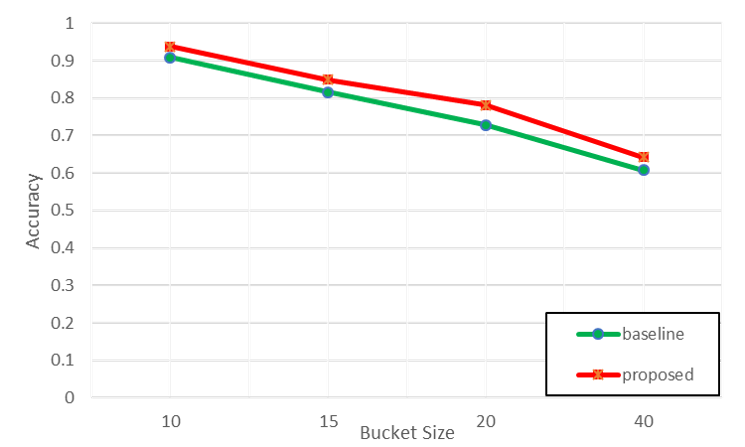
\includegraphics[width=.9\linewidth]{ACCU1.png}
    \caption{Accuracy vs. Bucket Size}
    \label{fig:sub1}
\end{subfigure}%
\begin{subfigure}{.5\textwidth}
    \centering
    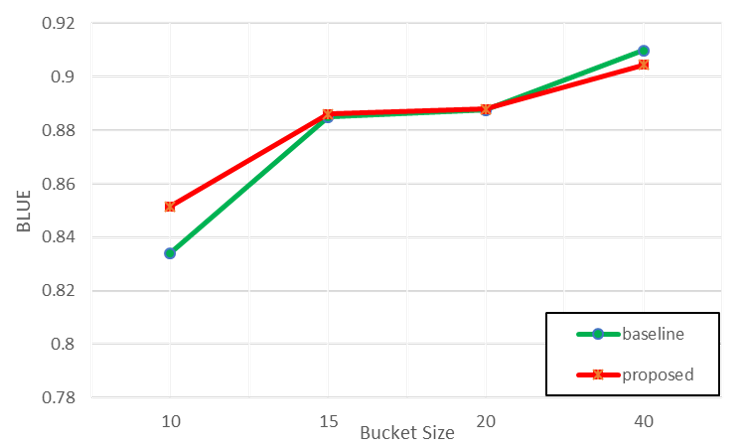
\includegraphics[width=.9\linewidth]{BLUE1.png}
    \caption{BLUE score vs. Bucket Size}
    \label{fig:sub2}
\end{subfigure}
\caption{Results of proposed model and baseline for different bucket size after 40000 times when coveraging.}
\label{fig:9}
\end{figure}
From Figure~\ref{fig:9}, we can notice that the trained GEC system outperforms this baseline for all bucket sizes in terms of accuracy. The GEC system also outperforms the baseline except only case in terms of BLEU score. This tells us that applying the seq2seq model with LSTM to a potentially errant writing sample would, on average, results in a more grammatically correct writing sample. 

In addition, how the performance of the trained model change with the number of iteration. If the performance of the trained model become worse at the large number region, we may need to do ``early stop'' trick for the training.
\begin{figure*}
    \centering
    \begin{subfigure}[b]{0.475\textwidth}
        \centering
        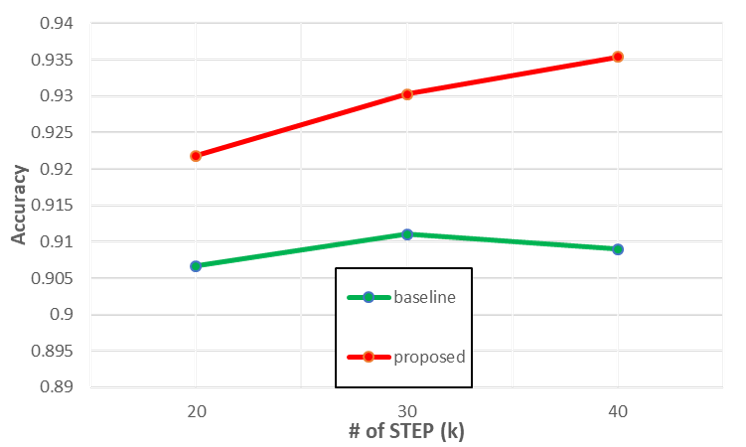
\includegraphics[width=\textwidth]{ACCU10.png}
        \caption[]%
        {{\small Accuracy vs. step number for Bucket size $= 10$}}    
        \label{fig:ACCU10}
    \end{subfigure}
    \hfill
    \begin{subfigure}[b]{0.475\textwidth}  
        \centering 
        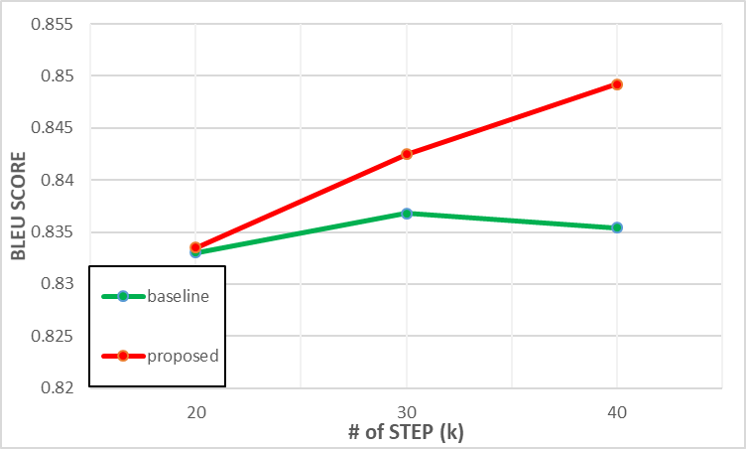
\includegraphics[width=\textwidth]{BLUE10.png}
        \caption[]%
        {{\small BlEU Score vs. step number for Bucket size $= 10$}}    
        \label{fig:BLUE10}
    \end{subfigure}
    \vskip\baselineskip
    \begin{subfigure}[b]{0.475\textwidth}
        \centering
        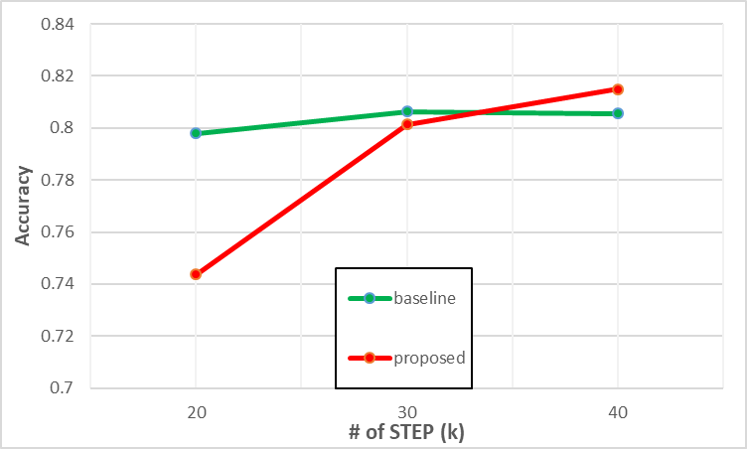
\includegraphics[width=\textwidth]{ACCU15.png}
        \caption[]%
        {{\small Accuracy vs. step number for Bucket size $= 15$}}    
        \label{fig:ACCU15}
    \end{subfigure}
    \hfill
    \begin{subfigure}[b]{0.475\textwidth}  
        \centering 
        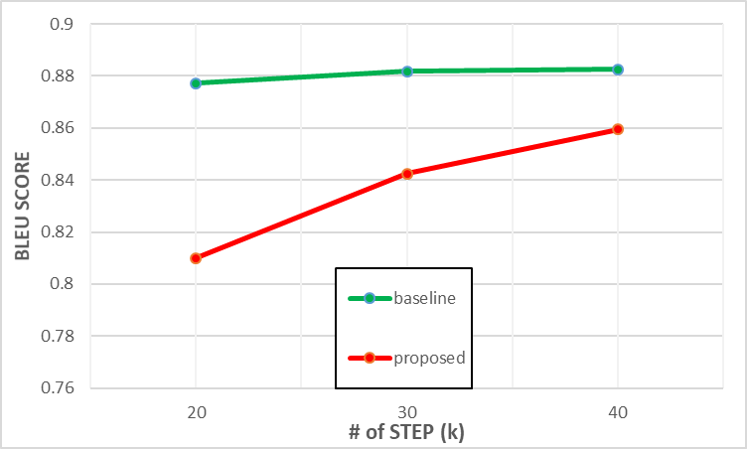
\includegraphics[width=\textwidth]{BLUE15.png}
        \caption[]%
        {{\small BlEU Score vs. step number for Bucket size $= 15$}}    
        \label{fig:BLUE15}
    \end{subfigure}
    \vskip\baselineskip
    \begin{subfigure}[b]{0.475\textwidth}
        \centering
        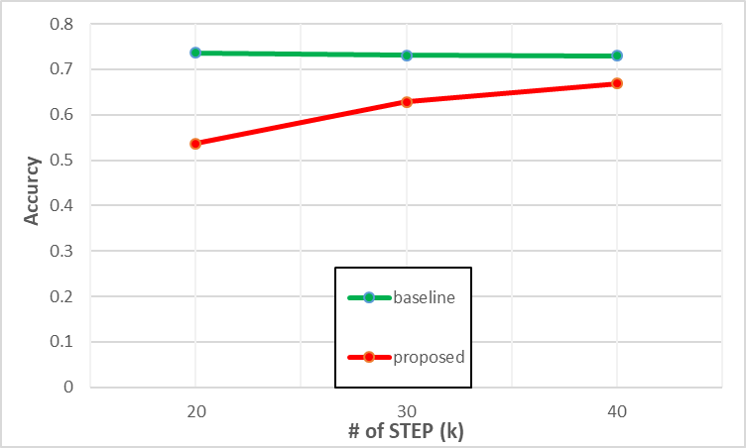
\includegraphics[width=\textwidth]{ACCU20.png}
        \caption[]%
        {{\small Accuracy vs. step number for Bucket size $= 20$}}    
        \label{fig:ACCU20}
    \end{subfigure}
    \hfill
    \begin{subfigure}[b]{0.475\textwidth}  
        \centering 
        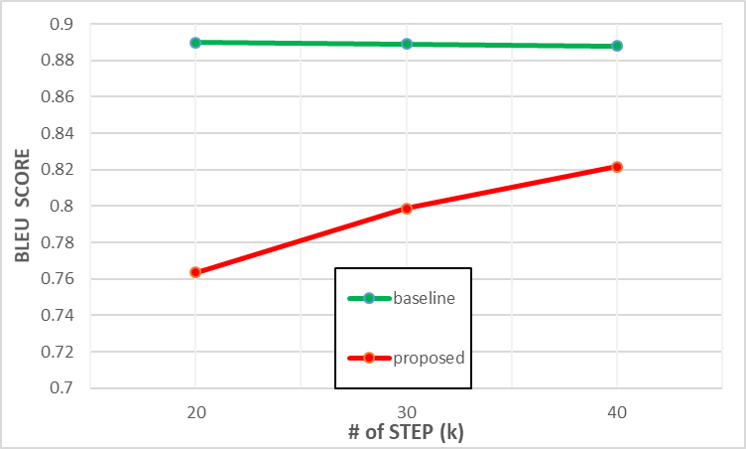
\includegraphics[width=\textwidth]{BLUE20.png}
        \caption[]%
        {{\small BlEU Score vs. step number for Bucket size $= 20$}}    
        \label{fig:BLUE20}
    \end{subfigure}
    \vskip\baselineskip
    \begin{subfigure}[b]{0.475\textwidth}   
        \centering 
        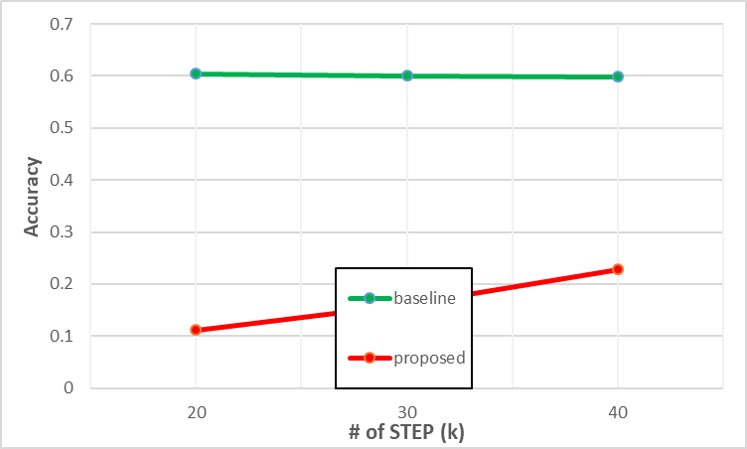
\includegraphics[width=\textwidth]{ACCU40.png}
        \caption[]%
        {{\small Accuracy vs. step number for Bucket size $= 40$}}    
        \label{fig:ACCU40}
    \end{subfigure}
    \quad
    \begin{subfigure}[b]{0.475\textwidth}   
        \centering 
        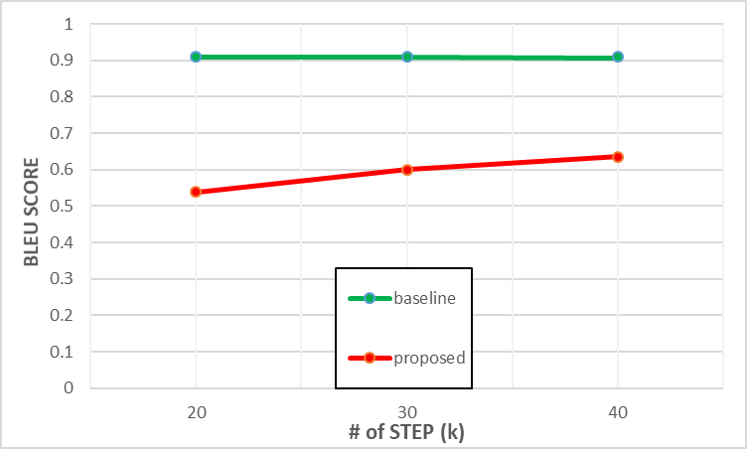
\includegraphics[width=\textwidth]{BLUE40.png}
        \caption[]%
        {{\small BlEU Score vs. step number for Bucket size $= 40$}}    
        \label{fig:BLUE40}
    \end{subfigure}
    \caption[]
    {\small Performance vs. step number for different Bucket size} 
    \label{fig:performance}
\end{figure*}
The results are shown in Figure~\ref{fig:performance}.
From Figure~\ref{fig:performance}, we can get the following conclusions.
\begin{itemize}
    \item The performance of the trained models are better for the smaller bucket size. From Figure~\ref{fig:performance} and Figure~\ref{fig:9}, we can see that the trained model of bucket size $=10$ can outperforms the baseline for different iteration step numbers. For the hyper-parameter bucket size, it is recommended to set bucket size to smaller value instead a larger one.
    \item As the number of iteration step increases, the performance of the trained model become better. It means that the model does not show overfit within 40000 steps.
    \item The trained model is not always better than the baseline. From Figure~\ref{fig:performance}, the performance of the trained model is worse than the baseline in six subfigures. Thus, the hyper-parameters should be carefully tuned.
\end{itemize}

\section{Examples}
The following Figure shows some case we test for the GEC system. This shows that the GEC system can Decoding a sentence with a missing article. From the figure, we can also see that there are still many typos the GEC system cannot detect. However, overall, the performance of the trained GEC system is acceptable.
\begin{figure}[ht]
    \centering
    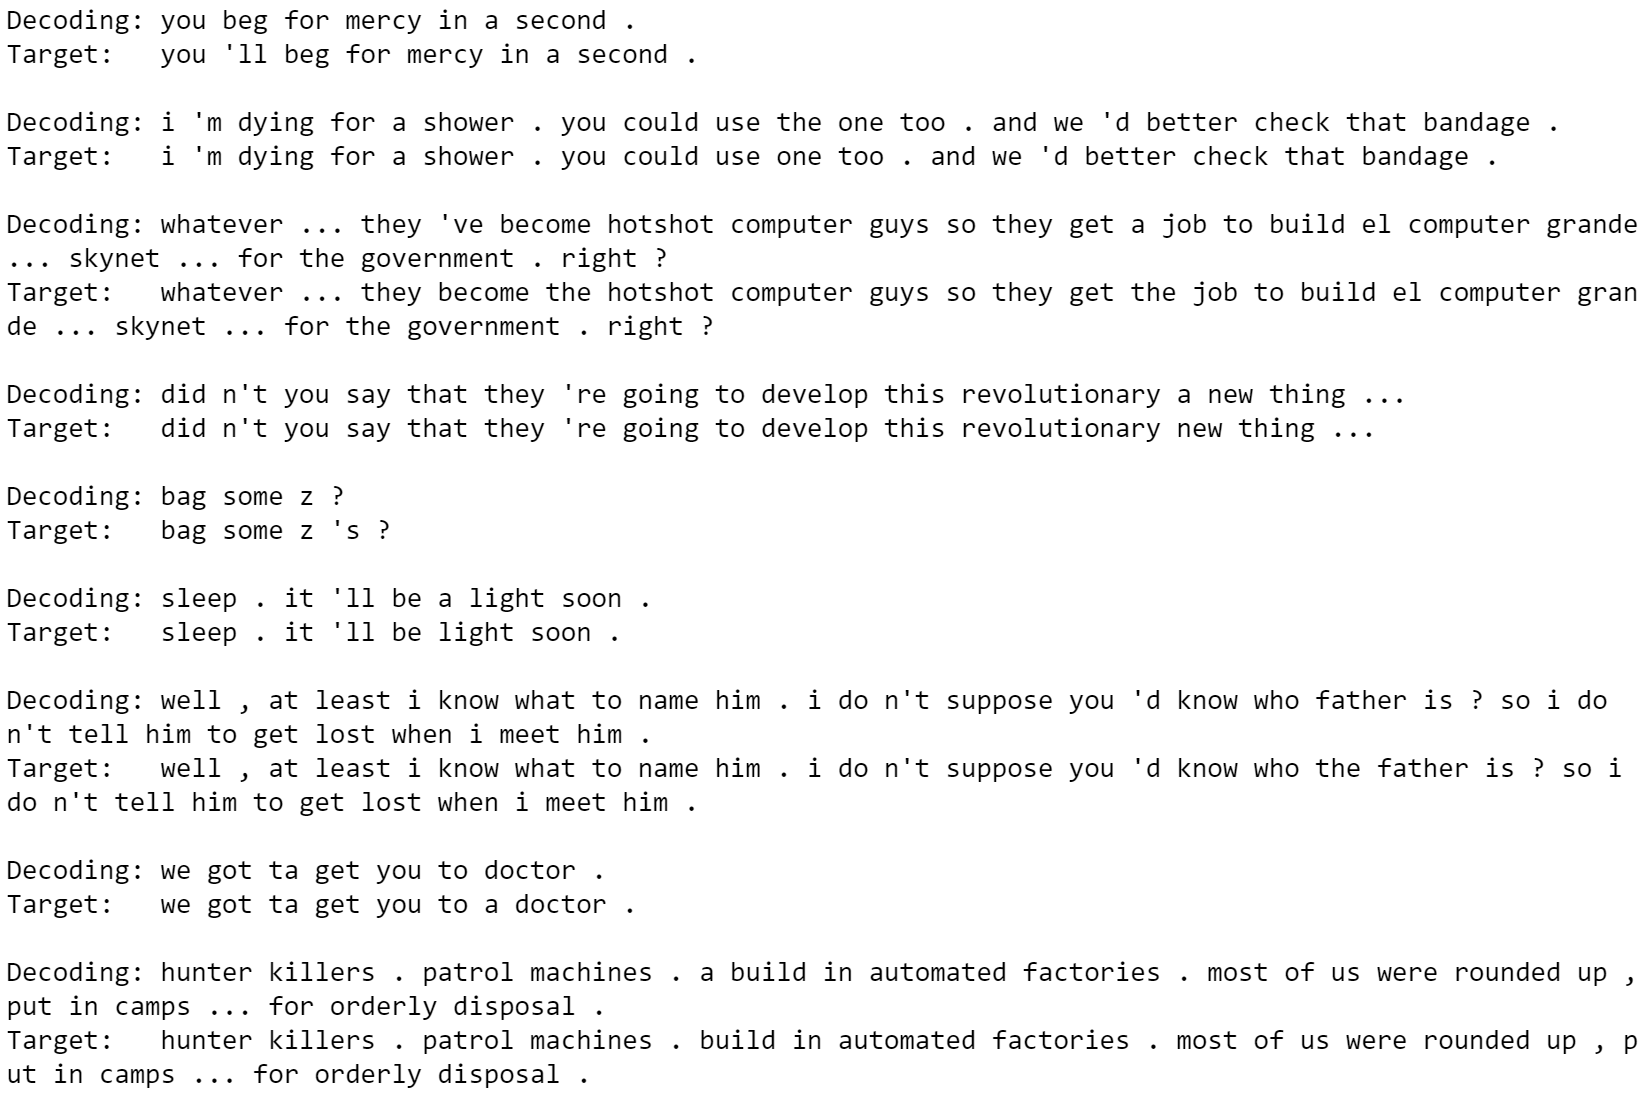
\includegraphics[width=0.8\textwidth]{testcase.png}
    \caption{Test Cases.}
    \label{fig:10}
\end{figure}